
A directional coupler is composed of two straight waveguides at a distance $g$. The width of the waveguides can either be the same (symmetric coupler), as represented in Fig. \ref{fig:wg_design}, or different (asymmetric coupler).

\begin{figure}[H]
    \centering
    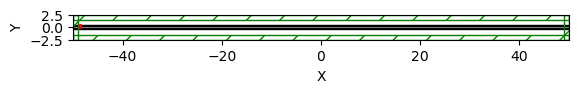
\includegraphics[width=0.8\linewidth]{Figures/wg_design.png}
    \caption{Design of the simulation of a directional coupler. Two parallel symmetric waveguides of width \(w=0.5\ \mu m\) and separated by a gap \(g=0.1\ \mu m\). The guides are made from a material with dielectric constant \(\varepsilon = 12.25\). The simulation is done at resolution \(r=10\) in a simulation space with PML of thickness \(1\ \mu m\).}
    \label{fig:wg_design}
\end{figure}

The directional coupler allows to exchange field from one waveguide to another thanks to the evanescence field. If the two waveguides are identical there is a total exchange of field from one to the other and this happens at the coupling length $\ell_C$. In Fig. \ref{fig:wg_field_fit} is reported the amplitude of the electric field oscillations inside the two guides. The envelope of the field shows how the field is exchanged from one guide to the other.

To evaluate the coupling length two methods were tested. At first, the coupling length was evaluated by finding the minima of the envelope and computing half of their distance. This method isn't very robust and returns wrong results on limit cases.

A second possibility is to evaluate the FFT of the envelope and extract from it a guess on the frequency of the amplitude variation. Using this guess fit the envelope with the function in Eq. \ref{eq:field_fit}
\begin{equation} \label{eq:field_fit}
    f(x) = A \cdot \sin^2{(\omega t + \phi)}
\end{equation}
where \(A\) is the amplitude, \(\omega\) the angular frequency and \(\phi\) the phase.

The result of the fit is reported in Fig. \ref{fig:wg_field_fit}. The fit is done on the electric field in the upper waveguide and it is reported with a $\pi / 2$ shift on the lower waveguide field. From the image, it's clear that the field in the two guides has the same frequency and amplitude while the only difference is the phase.

\begin{figure}[H]
    \centering
    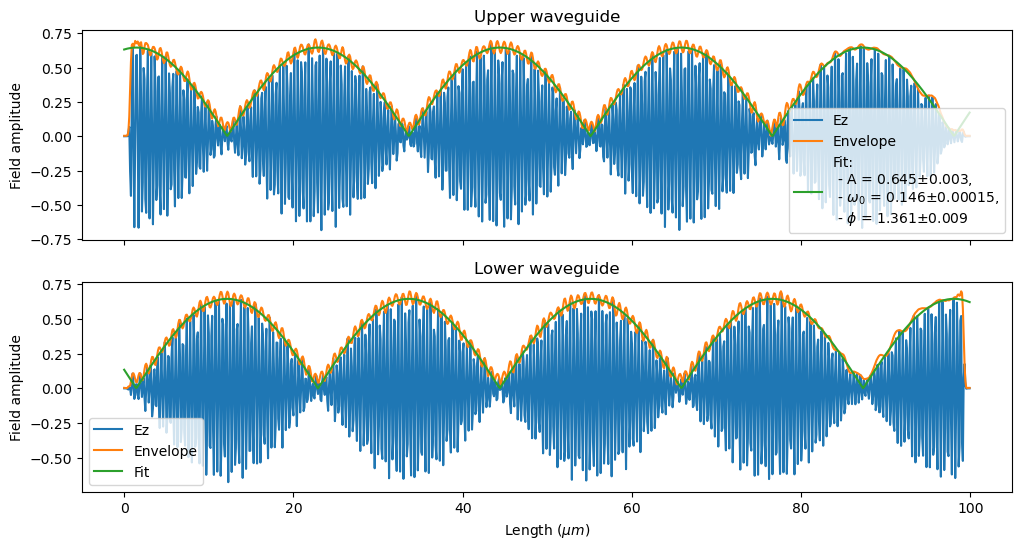
\includegraphics[width=0.6\linewidth]{Figures/wg_field_fit.png}
    \caption{Electric field oscillating along the $z$ axis inside the waveguide and its envelope. The envelope is fitted with the function in Eq. \ref{eq:field_fit}.}
    \label{fig:wg_field_fit}
\end{figure}

\subsection{Symmetric directional coupler}

The difference between a symmetric and asymmetric directional coupler is the amount of transferred energy from one guide to the other. In the symmetric coupler all the field is transferred from one guide to the other while for the asymmetric one only a part of the field is transferred. 

\begin{figure}[H]
    % \centering
    % \begin{subfigure}[b]{0.45\linewidth}
        \centering
        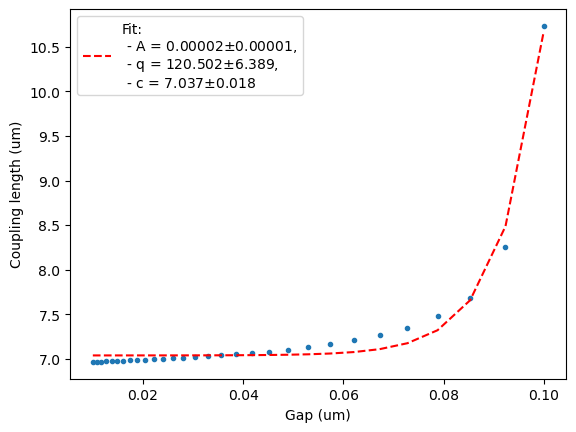
\includegraphics[width=0.5\linewidth]{Figures/wg_coupling_vs_gap.png}
        \caption{Repeated simulation at different values of \(g\) ranging from \(0.01\ \mu m\) to \(0.1\ \mu m\). The dependence of the coupling length on the gap is fitted with the function \(f(x) = A \cdot e^{qg} + c\) as suggested by Eq. \ref{eq:coupling_dependence}.}
        \label{fig:wg_coupling_vs_gap}
        % \end{subfigure}
        % \hfill
        % \begin{subfigure}[b]{0.45\linewidth}
            %     \centering
            %     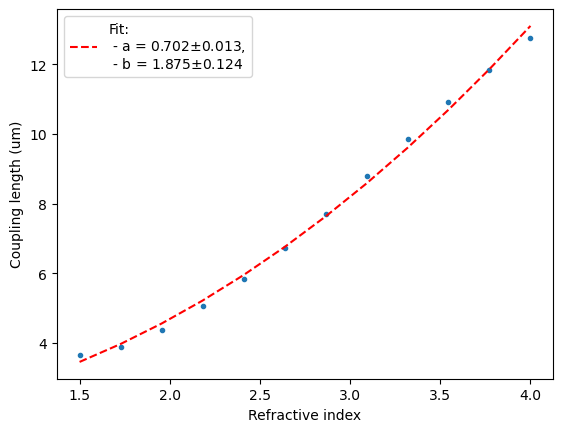
\includegraphics[width=\linewidth]{Figures/wg_coupling_vs_index.png}
            %     \caption{}
            %     \label{fig:wg_coupling_vs_index}
            % \end{subfigure}
\end{figure}
        
The coupling length is defined as $\ell_C = \pi / 2\alpha$ where $\alpha$ is the coupling constant between the guides. For the symmetric coupler the coupling constant depends on several parameters\cite{photonics_book}, among which are the width of the waveguides, the gap between them and the refractive index contrast between the guiding material and the substrate. A more precise dependence from the gap is reported in Eq. \ref{eq:coupling_dependence}
\begin{equation} \label{eq:coupling_dependence}
    \alpha \propto e^{-q\cdot g} 
\end{equation}
where \(g\) is the gap width and \(q\) depends on the effective wavevector, the substrate refractive index and the frequency of the field\cite{photonics_book}.

The simulation was repeated for different values of the gap and the coupling length was extracted with the FFT. The data produced are reported in Fig. \ref{fig:wg_coupling_vs_gap} together with an exponential fit. The agreement with the fit is quite good but it shows that a linear dependence is missing on the base of the exponential.
        
\subsection{Asymmetric directional coupler}

For an asymmetric directional coupler, not all the power is transferred from one guide to the other as can be seen in Fig. \ref{fig:wg_field_asymm}.

\begin{figure}[H]
    \centering
    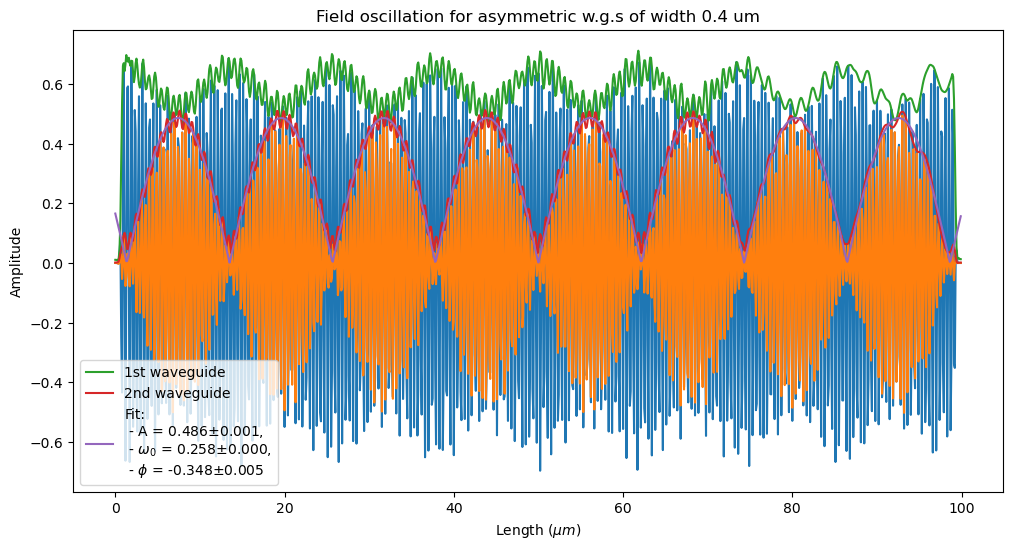
\includegraphics[width=0.8\linewidth]{Figures/wg_field_asymm.png}
    \caption{Electric fields oscillating along the z-axis inside the asymmetric waveguides and their envelopes. The fields were produced by the coupling of two straight waveguides the first one (top waveguide) of width \(0.5\ \mu m\) while the second one (bottom waveguide) of width \(0.4\ \mu m\). The envelope of the field in the bottom waveguide is fitted with the function in Eq. \ref{eq:field_fit} to obtain the coupling length.}
    \label{fig:wg_field_asymm}
\end{figure}

The coupling length can be influenced also by this asymmetry, so the simulation was repeated by changing just the width of the bottom waveguide and the result is represented in Fig. \ref{fig:wg_coupling_vs_asymm}, showing a clear dependence of the coupling length from the asymmetry. The last point in Fig. \ref{fig:wg_coupling_vs_asymm} corresponds to the symmetric coupling.

But another important quantity to consider in case of asymmetry is the power transfer, namely how much of the power in the first guide is transferred to the second guide. The power is computed as the square amplitude of the field in the bottom guide and then normalized for the maximum power in the top guide to obtain the ratio. The ratio changes with the distance from the source, so only the maximum of the ratio is considered and reported in Fig. \ref{fig:wg_power_vs_asymm} as a function of the asymmetry. Again it's clear that the ratio of transferred power depends on the asymmetry in particular the maximum ratio is obtained in the symmetric configuration (last point).

\begin{figure}[H]
    \centering
    \vfill
    \begin{subfigure}[b]{0.48\linewidth}
        \centering
        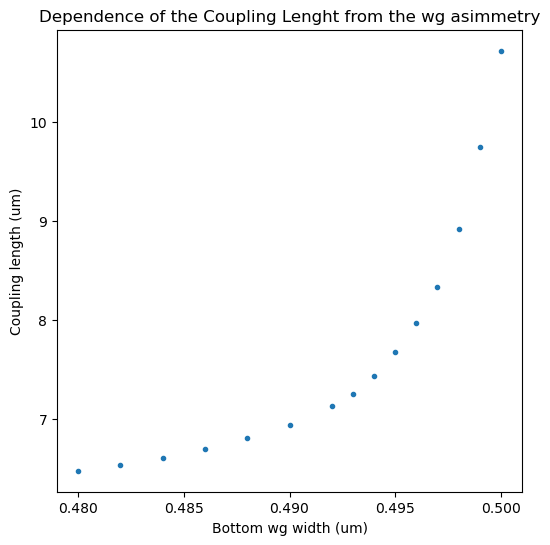
\includegraphics[width=\linewidth]{Figures/wg_coupling_vs_asymm.png}
        \caption{Dependence of the coupling length on the width asymmetry.}
        \label{fig:wg_coupling_vs_asymm}
    \end{subfigure}
    \hfill
    \begin{subfigure}[b]{0.48\linewidth}
        \centering
        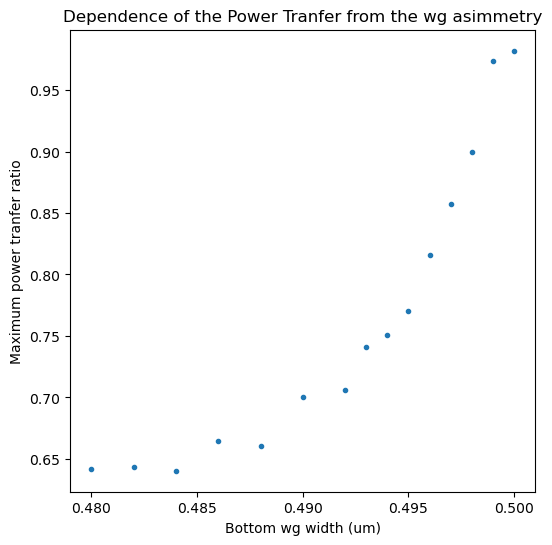
\includegraphics[width=\linewidth]{Figures/wg_power_vs_asymm.png}
        \caption{Dependence of the maximum power transfer ratio on the width asymmetry.}
        \label{fig:wg_power_vs_asymm}
    \end{subfigure}
    \caption{Simulations repeated at different widths of the bottom waveguide ranging from \(0.48\ \mu m\) to \(0.5\ \mu m\). For each simulation, the coupling length and the maximum power transfer ratio are evaluated to show their dependence on the width asymmetry.}
\end{figure}